\documentclass{article}
\usepackage{amsmath}
\usepackage{amsfonts}
\usepackage{amssymb}
\usepackage{graphicx}
\usepackage[absolute,overlay]{textpos}

\begin{document}

\begin{textblock*}{3cm}(0.5cm,1cm) % {width}(xcoord, ycoord)
    
\includegraphics[width=3cm]{imagen2.png}
\end{textblock*}
\title{Modelo Matemático para la Planificación de Inversiones}
\author{Melani Forsythe Matos \\ 312 Carrera Ciencias de la Computación}
\date{}

\maketitle

\section*{Introducción}
Dado un conjunto de 10 proyectos, donde cada proyecto $i$ tiene:
\begin{itemize}
    \item Beneficio esperado $c_i$.
    \item Costo $b_i$.
    \item Requerimiento de recurso $r_i$.
\end{itemize}

El objetivo es seleccionar los proyectos que maximicen el beneficio total, sujeto a las restricciones de presupuesto y disponibilidad de recursos.

\subsection*{Modelo Matemático}

\textbf{Variables de decisión}:
\[
x_i =
\begin{cases}
1, & \text{si el proyecto $i$ es seleccionado}, \\
0, & \text{en caso contrario}.
\end{cases}
\]

\textbf{Función objetivo}:
\[
\text{Maximizar: } Z = \sum_{i=1}^n c_i x_i
\]
Donde $Z$ representa el beneficio total esperado.

\textbf{Restricciones}:
\begin{enumerate}
    \item Restricción de presupuesto:
    \[
    \sum_{i=1}^n b_i x_i \leq B
    \]
    Donde $B$ es el presupuesto total disponible.
    
    \item Restricción de recursos:
    \[
    \sum_{i=1}^n r_i x_i \leq R
    \]
    Donde $R$ es el total de recursos disponibles.
    
    \item Restricción de selección binaria:
    \[
    x_i \in \{0, 1\} \quad \forall i
    \]
\end{enumerate}

\section*{Aplicación del Modelo a un Conjunto de Datos}

Aplicando este modelo a un conjunto de datos con los siguientes valores:
\begin{itemize}
    \item Beneficios: [100, 200, 150, 300, 250, 400, 350, 500, 450, 600]
    \item Costos: [50, 80, 60, 100, 90, 120, 110, 140, 130, 160]
    \item Recursos: [60, 80, 70, 90, 85, 100, 95, 110, 105, 120]
    \item Presupuesto total: 700
    \item Recurso total: 800
\end{itemize}

Obtenemos los siguientes resultados:

\begin{figure}[h!]
    \centering
    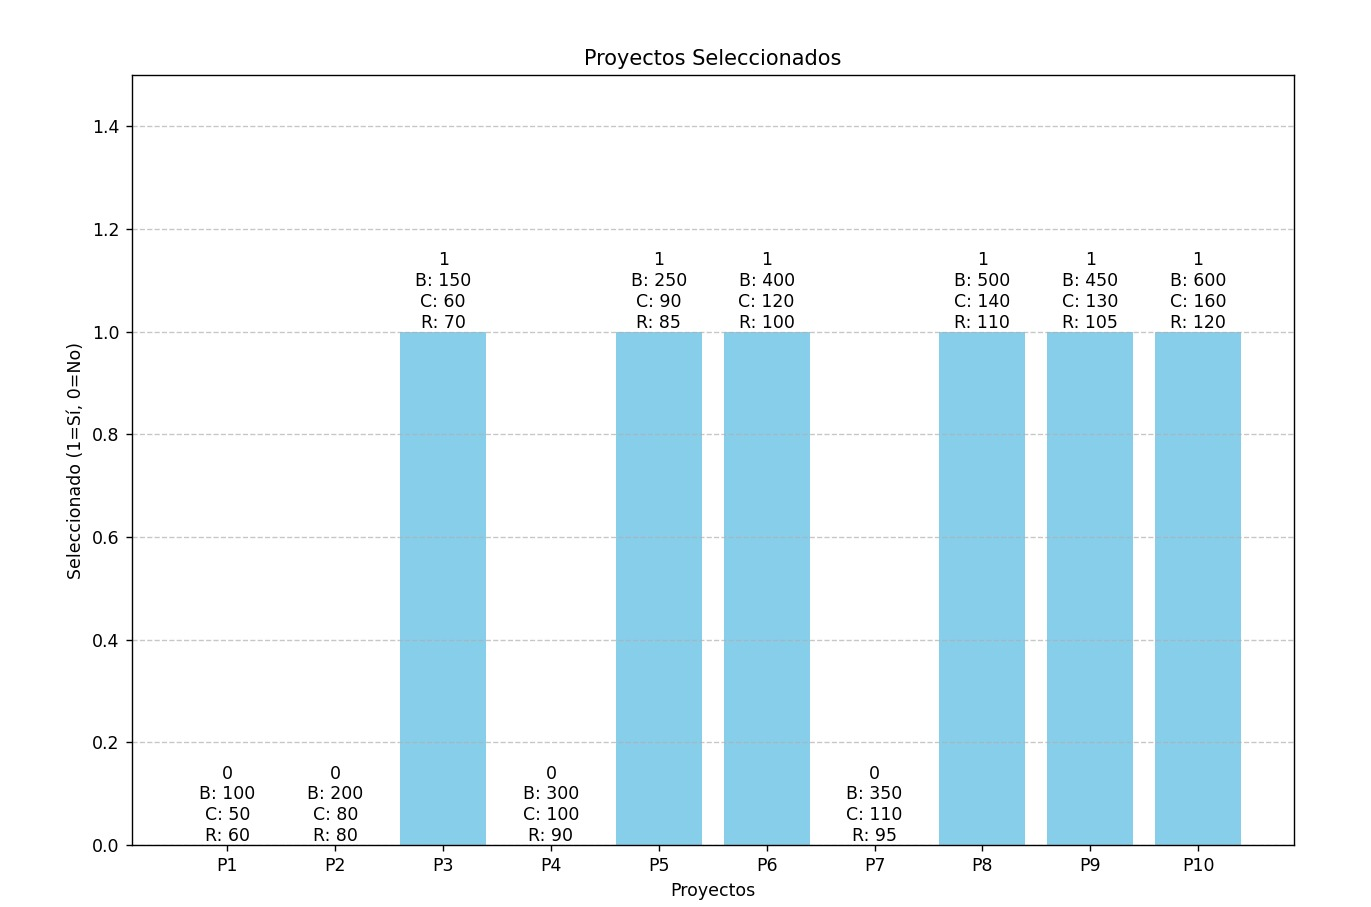
\includegraphics[width=0.8\textwidth]{resultados.png}
    \caption{Proyectos Seleccionados}

\end{figure}


\end{document}
